\subsection{Trusting the beacon}%
\label{sub:trusting_the_beacon}

We propose two scenarios, which can be used to describe the users trust assumptions towards the beacon.
In both of these scenarios, we focus on a given user named Alice, while all other users are regarded as potentially colluding adversaries with malicious intent.
The only assumption about these adversaries, is that they can interact with the beacon in the same manner as Alice; i.e.\ send inputs to the beacon.

Because network latency is dependent on many variables in a system and virtually impossible to verify, we assume the latency is non existent.
As a consequence of this, Alice will assume that any inputs she sends is received immediately by the beacon, and vice versa --- any message from the beacon is received instantly by her.
This means that the beacon will not be able to claim different timings than what Alice observes.

\paragraph{Scenario \#1 --- An honest operator.}
This is the best case scenario for Alice.
The operation of the beacon is honest, which means that
\begin{eletterate*}
\item the beacon operator will accept all inputs, i.e.\ not exclude any;
\item the commitment is published as soon as possible, i.e.\ right after a batch of inputs has been processed; and
\item the output and proof is published immediately after the computation is done.
\end{eletterate*}

With this honest beacon, Alice knows exactly how long the computation took, and can trust the output to not be manipulated in any predictable way.
However, assuming honesty is not advised, since it leaves Alice vulnerable by exploiting this trust.
If Alice trusts the beacon operator to be honest, she will not suspect them to act according to the following scenario.

\paragraph{Scenario \#2 --- A malicious operator.}
This is the worst case scenario for Alice; a beacon operator, which is trying to choose the output, yet still make it seem valid for Alice.
The malicious operator will not resort to excluding Alice's input, since they are interested in fooling her to trust a forged output.
Moreover, the malicious operator should be expected to collude with all other users against Alice --- she is effectively alone in wonderland.

When the operator is acting malicious they will try to manipulate the output, while displaying correct operation outwards.
This means that Alice still will receive a commitment, output, and proof, which she can use to verify the correctness of the output.
As will she received these messages at virtually the same timing as described in the honest operator scenario.
The main difference here, is that Alice should not assume correlation between timings of received messages, and timings of beacon process.

Assume the following behaviour of a malicious operator:
\begin{eletterate*}
\item the beacon operator will stop input collection after receiving Alice's input;
\item they will attempt to publish the commitment, output, and proof when it is expected by Alice;
\item the operator will use unlimited resources to pre-compute possible outputs to seemingly valid commitments;
\item the operator will use pseudo inputs to affect outcomes, which will give the impression of input collection after Alice's input;
\item out of the pre-computed outputs, the malicious operator will choose the one which benefits them the most.
\end{eletterate*}

In this scenario the operator will effectively carry out a last-draw attack against Alice.
Moreover, if the malicious operator cannot compute a outcome which they deem beneficial, they are capable of claiming disrupted operation before publishing any commitment.
This will leave Alice without any output, but she will not be able to know if the operator was malicious or disrupted by a third party adversary.
Hereby deploying a withholding-attack on Alice.

\subsection{Probabilistic Trust}%
\label{sub:probabilistic_trust}
In our approach to a randomness beacon, we want to push beyond the need for honest operators, and naïve users.
To achieve this, we first need to quantify trusting the beacon and then determine thresholds for reasonable behaviour.
This effectively will provide a measure of probabilistic trust, where users much decide for themselves, if the probability of honest operation is adequate.

We present an property, which if satisfied, says that the user can trust that the beacon operator is not capable of fooling them.
The property is true, if the user determines that nobody will be able to compute the delay function in the time between they sent their input and received the commitment.
This can be condensed to:
\begin{equation}
    t_{INPUT} - t_{COMMITMENT} < T_{DELAY FUNCTION}
\end{equation}
given that $t_{INPUT}$ is the time when the user sent the input, $t_{COMMITMENT}$ is when the user received the commitment, and $T_{DELAY FUNCTION}$ is the fastest computation of the given delay function.
This tells us that for users to be more likely to trust a beacon, the time between they send their input and receive the commitment, must be significantly smaller than the time between the commitment and the output.
In fact, it must be smaller than the shortest time a given user thinks the operator could be able to compute the delay function.

Taking this into consideration we present a beacon operation protocol, which can be adjusted to increase or decrease this limit.
The operation must be sequential, which means that we must collect input before computing the delay function.
However, because we want to spend more time computing, than we are collecting input, a strictly sequential beacon will contain dead spots, where no user is submitting input.
This may be acceptable in some scenarios, but we want to design a beacon which always accepts inputs, and which wont be suspected of malicious operation.
To achieve this we parallelize the beacon protocol, meaning that several delay functions will run in parallel but offset in time, and using different input.
In~\cref{fig:beacon_parallel_timeline} we illustrate this.

\begin{figure}
    \centering
    \footnotesize
    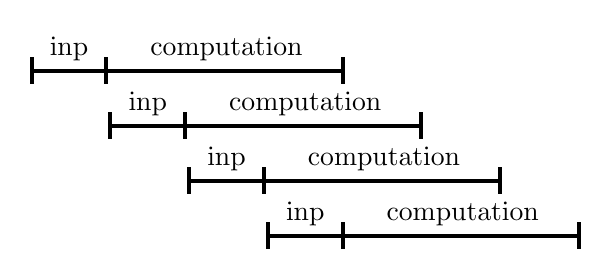
\begin{tikzpicture}
    \foreach \x in {0, 1, 2,...,3} {
        \draw[|-|, black, line width=0.5mm] (\x,-\x*0.7) to (\x+1,-\x*0.7);
        \path (\x,-\x*0.7) -- (\x+1,-\x*0.7) node [midway, above] {inp};
        \draw[-|, black, line width=0.5mm] (\x+1,-\x*0.7) to (\x+4,-\x*0.7);
        \path (\x+1,-\x*0.7) -- (\x+4,-\x*0.7) node [midway, above] {computation};
    }
    \end{tikzpicture}
    \caption{Parallelized beacon protocol, with offset input collection and overlapping computation.}\label{fig:beacon_parallel_timeline}
\end{figure}

\begin{figure}
    \centering
    \footnotesize
    \begin{tikzpicture}
    \pgfdeclarelayer{background}
    \pgfsetlayers{background,main}
    \draw[|-ss, line width=0.5mm, black] (0,0.7) to (8.3,0.7);
    \path (0,0.7) -- (8,0.7) node [midway, above] {Input Collection Stream};

    \foreach \x in {0, 1, 2} {
        \begin{pgfonlayer}{background}
            \draw[latex reversed-, dotted, black, line width=0.2mm] (\x+1,0.7) to (\x+1,-\x*0.7);
        \end{pgfonlayer}
        \draw[-o, GoogleIndigo, line width=0.5mm] (\x+1,-\x*0.7) to (\x+4,-\x*0.7);
        \path (\x+1,-\x*0.7) -- (\x+4,-\x*0.7) node [midway, above] {\contour{white}{Computation}};
    }
    \foreach \x in {3, 4} {
        \begin{pgfonlayer}{background}
        \draw[latex reversed-, dotted, black, line width=0.2mm] (\x+1,0.7) to (\x+1,{-(\x-3)*0.7});
        \end{pgfonlayer}
        \draw[-o, GoogleIndigo, line width=0.5mm] (\x+1,{-(\x-3)*0.7}) to (\x+4,{-(\x-3)*0.7});
        \path (\x+1,{-(\x-3)*0.7}) -- (\x+4,{-(\x-3)*0.7}) node [midway, above] {\contour{white}{Computation}};
    }

    \begin{pgfonlayer}{background}
    \draw[latex reversed-, dotted, black, line width=0.2mm] (6,0.7) to (6,-0.7*2);
    \end{pgfonlayer}
    \draw[-ss, GoogleIndigo, line width=0.5mm] (6,-0.7*2) to (8.3,-0.7*2);

    \begin{pgfonlayer}{background}
    \draw[latex reversed-, dotted, black, line width=0.2mm] (7,0.7) to (7,0);
    \end{pgfonlayer}
    \draw[-ss, GoogleIndigo, line width=0.5mm] (7,0) to (8.3,0);

    \begin{pgfonlayer}{background}
    \draw[latex reversed-, dotted, black, line width=0.2mm] (8,0.7) to (8,-0.7);
    \end{pgfonlayer}
    \draw[-ss, GoogleIndigo, line width=0.5mm] (8,-0.7) to (8.3,-0.7);

    \end{tikzpicture}
    \caption{Parallelized beacon protocol, with input collection stream and overlapping computation.}\label{fig:beacon_parallel_timeline_real}
\end{figure}
